% \Huge

With the tools developed in the previous chapter, and the perfect reconstruction serving as an upper limit for reconstruction, we are ready to dive into realistic reconstruction methods. In Section 1.2.2 we outlined different reconstruction methods used in practice. This project will study reconstruction within the Zel'dovich approximation. We will use particle velocities to attempt to track their motion back in time. As before, the density field will be carried along with the particles.

\section{The Zel'dovich Approximation}

\subsection{Background}

The central object of Lagrangian Perturbation Theory is the displacement field $\Psi(\textbf{q})$ which maps the initial particle positions expressed by the Lagrangian coordinate $\textbf{q}$ to the final comoving Eulerian particle positions $\textbf{x}$ (\cite{Bernardeau_PT}):
\begin{equation}
     \textbf{x}(t) = \textbf{q} + \Psi(\textbf{q}, t)
\end{equation}

The first order approximation to this equation leads to a separation of variables $\textbf{q}$ and $t$ (\cite{1993sfu..book.....P}). After adding the expanding background we obtain the Eulerian particle positions as:
\begin{equation}
    \textbf{r}(t) = a(t) \textbf{x}(t) = a(t) [\textbf{q} + b(t) \textbf{p}(\textbf{q})]
    \label{eq:2.2}
\end{equation}
Where $\textbf{r}(t)$ is the Eulerian coordinate, and $a(t)$ is the scale factor.

This approximation was first proposed by~\cite{1970A&A.....5...84Z} and it now carries his name, as the Zel'dovich Approximation (ZA). It only works for scales much smaller than the horizon, where Newtonian analysis is possible. However, as our purpose is to study the growth of structure on scales smaller than the BAO, this approximation is a very good starting point. 

An important detail is that the ZA (up to a point) works even in the non-linear regime. This regime is defined in terms of the overdensity $\delta$. When $\delta \sim 1$ we enter the non-linear regime. Standard Perturbation Theory generally breaks down at this point. However, by switching to a description in terms of the particle trajectories, we can reach non-linear density contrasts without the particles being perturbed too much (\cite{1993sfu..book.....P}).

On a final note, the ZA is very good at predicting the loss of correlation between the initial and the final density fields (e.g.~\cite{Pontzen_paired_simulations}). This is the reason we have chosen this framework for our reconstructions.


\subsection{Tracing particles back}

The key ingredient that we will use to perform realistic reconstructions is the peculiar velocity field. The idea behind the Zel'dovich approximation is to calculate a linear displacement field (we refer to this field as the Zel'dovich offset) based on the current peculiar velocities while taking into account the Hubble flow. 

The peculiar velocity predicted by the ZA (\cite{1993sfu..book.....P}) is given by:
\begin{equation}
    \textbf{V}(t) \equiv a(t)\frac{d\textbf{x}}{dt}    
\end{equation}
Using Equation~\ref{eq:2.2}, we arrive at a peculiar velocity given by:
\begin{equation}
    \textbf{V} = a(t)\dot{b}\textbf{p}(\textbf{q})
\end{equation}
Finally, bringing the displacement field back ($\Psi(\textbf{q},t) = b(t) \textbf{p}(\textbf{q})$), and switching variables to redshift we obtain:
\begin{equation}
    \Psi_z(\textbf{q}) = \frac{\textbf{V}(\textbf{q})}{a(z)} \times \frac{b(z)}{f(z)}
    \label{eq:4.1}
\end{equation} 
Where $b(z)$ is called the linear growth factor and $f(z) = \dot{b}(z)$ is the rate of linear growth. To calculate these two, we use the integration methods implemented in \textit{Pynbody} (\cite{2013ascl.soft05002P}).

As we are interested in looking at the correlation between the reconstructed field  and the initial fields in our simulations (which are at $z=99$), we need to calculate the Zel'dovich offset up to $z=99$ only. In order to achieve this, we first used equation~\ref{eq:4.1} to calculate the offset starting from the redshift $z$ of the snapshot ($\Psi_z$). After that, we used the same equation to approximate this offset from $z=99$ ($\Psi_{99}$) using the same velocity field. The displacement field we are after is then given by:

\begin{equation}
    \Psi(\textbf{q}) = \Psi_z(\textbf{q}) - \Psi_{99}(\textbf{q})
    \label{eq:4.2}
\end{equation}


\subsection{The Reconstruction}

We first start out in our investigation by performing a reconstruction using the Zel'dovich offset calculated directly from the particle velocities in each snapshot. The methodology of the reconstruction resembles the perfect reconstruction. We first measure the density field at the particle positions in a snapshot, and then we apply the Displacement field $\Psi(\textbf{q})$ to move the particles. The density field is carried along. After that, \textsc{GenPK} is used to measure the cross power-spectra of the reconstructed field with the initial ($z=99$) field. This method is still unrealistic as we are using perfect knowledge of all the particle velocities, however it is the first step in our method. Therefore, we want to gain an understanding of how it performs and what are its limitations.

\begin{figure}
    \centering
    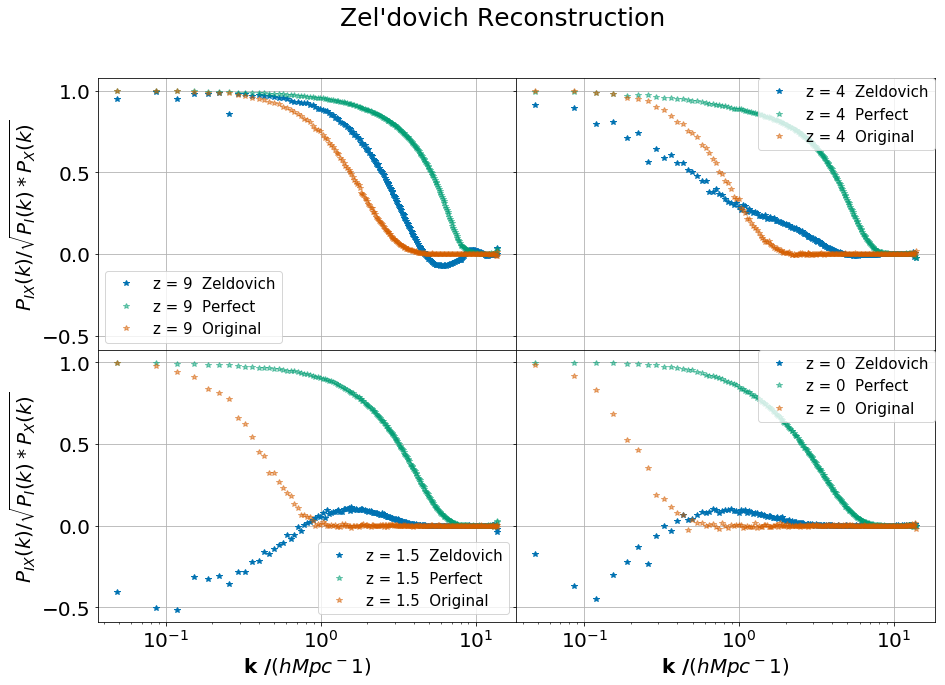
\includegraphics[width=1\columnwidth]{images/realRecon/zeld.png}%
    
    \caption{
    Normalized cross-spectra between the Zel'dovich reconstruction and the initial field. The original and perfect reconstruction correlations are also present to show us where we started and what the limit is. This reconstruction was performed by linearly moving the particles back in time (using the Zel'dovich approximation). As we apply the linear approximation directly to the particle velocities, this gives a good indicator of the regime we are in at that redshift. We see the reconstruction work very well when starting from $z=9$, which indicates we are still in the quasi-linear regime there. However, as time progresses (lower redshift) the correlation breaks down even on the largest scales, indicating we are mostly in the non-linear regime. 
    }
    
    \label{fig:4.1}
\end{figure}

The results of this reconstruction (we call it the Zel'dovich reconstruction) can be seen in Figure~\ref{fig:4.1}. We again look at the normalized cross-spectra between this reconstruction and the initial density field. To give us a better understanding of how well this method works, the original correlation and the perfect reconstruction are also present. The figure presents the reconstruction starting from four different snapshots in the redshift interval $z=9$ to $z=0$.

The reconstruction starting at $z=9$ gives very good results, bringing the decorrelation scale to an intermediate step between the original and the perfect reconstruction. At this redshift most particles are still in the quasi-linear regime, so this result is not surprising. An interesting feature is the small anti-correlation obtained at large $k$. This effect is most likely due to particles in non-linear regimes which are past shell-crossing. To understand what gives rise to this anti-correlation, consider two fronts of matter collapsing towards each other. After shell crossing there will be a turn-around as the two evolve into a single filament. If we linearly track these velocities back, we are effectively going the wrong way. This will lead to an anti-correlation over the affected scales. For the $z=9$ reconstruction, this effect is very small, indicating that shell crossing has only occurred on the smallest scales, and that most particle motions can be well approximated with the linear regime. 

However, at lower redshifts most particles are in the non-linear regime. By still treating their motions as linear we are breaking even the correlation that was there to begin with. Figure~\ref{fig:4.1} shows the largest scales decorrelating as we move to reconstructions from lower redshifts, and even leading to anti-correlation. For the lowest redshifts, we see a small improvement in the correlation on intermediate scales, but anti-correlation on large scales. This result is much harder to understand. A possible explanation is an extension to the reasons presented above for the anti-correlation in the $z=9$ reconstruction. The effect of particles that are past shell crossing moving the wrong way increases with decreasing redshift. This might lead to the large scales also becoming anti-correlated. This effect should be studied further, however, we leave this for future works, as our aim in this project is to achieve a good reconstruction.

We found that the Zel'dovich approximation works very well when starting in the quasi-linear regime (e.g. from $z=9$). On the other hand, it is not a good reconstruction method at low redshift because most particles have non-linear velocities. In this case, higher orders of LPT could perform better. However, at this point it is hard to justify this pursuit from an observational stand point. In this section we have used the peculiar velocities of particles in our simulations. As the ultimate goal of any reconstruction technique is to be used in practice on real data, we need to consider the feasibility of our method. Observers usually detect a few galaxies over an $8-10$ Mpc scale (\cite{dodelson2003modern}), and any peculiar velocity measurements inevitably come with errors. This means that the Zel'dovich reconstruction we just performed is very unrealistic in practice. The goal of the rest of this chapter is to modify the Zel'dovich reconstruction to make it more realistic, and also to improve its performance at low redshift.

\section{Getting back to linear velocities}

In order to make the Zel'dovich approximation work for our reconstruction, we must somehow get back into the quasi-linear regime. As discussed in Chapter 2, matter tends to be collapsed into filaments at late times. This means individual particles have non linear velocities, but ensembles of particles might still move linearly. Our solution to the two problems outlined in the previous section is to use bulk velocities to calculate the Zel'dovich offset, instead of individual particle velocities.

We smooth particle velocities over 1 Mpc and 10 Mpc scales respectively before calculating the Zel'dovich offset. This means we are now considering bulk motions instead of particle motions. These bulk motions will hopefully provide a better start point when we calculate the Zel'dovich offset. This smoothing also improves the realism of our method. Currently, observers can maybe detect a few galaxies in a 10 Mpc bin, so by smoothing our velocity field over that scale, we simulate a more realistic scenario. The reason for attempting a separate reconstruction using velocities smoothed over 1 Mpc scales is twofold. Firstly, we want to understand the effect of the velocity smoothing scale on the reconstruction. Secondly, we use the 1 Mpc case as a test for what could be achieved with improving technology and a better handling of systematics which could be useful for the next generation of Galaxy Surveys.

To perform these reconstructions, we first split a simulation into bins of a given size: $(1 Mpc)^3$ or $(10 Mpc)^3$. We then use the positions of the particles to identify the bin they are in. After that, an average velocity over the particles in each bin is calculated. This average velocity is assigned to the centre of the bin. In this manner, we construct a three-dimensional grid which contains a measure of the average velocity field. Finally, we use this average velocity field to linearly interpolate the value of the velocities at the particle positions. Particle velocities are therefore smoothed over the scales of interest. Using these new velocities, the Zel'dovich reconstruction is performed as outlined in the previous section.

To further improve the practicality of our method, we also attempt a second type of velocity smoothing. We perform all the steps outlined above to create an average velocity field, but this time we use smaller bins: $(0.5$ Mpc$)^3$ in size. We then use a Gaussian Filter to smooth this field over the scales of interest (1 Mpc and 10 Mpc respectively). From here, the procedure carries on as outlined above. However, an observer would only detect a few galaxies over a 10 Mpc scale. Also, on these small scales, velocities are most likely still in the non-linear regime. This leads us to perform the Gaussian smoothing over larger scales.

Before we move on to the results, an interesting side effect that should be mentioned showed up during the reconstruction. The nature of our method implies that we are creating coherent movements of particles. This coherent movement leaves large gaps in our reconstructed density field (regions where the density field is equal to 0). These gaps become a problem when we want to take the logarithm of the density field as discussed in Chapter 2. When calculating the density field, \textit{Pynbody} uses a smoothing kernel which normally fills in these gaps. However, this method uses N nearest neighbours to calculate the smoothing scale in a region. Normally, there still are a few particles even in the largest voids. These particles will have very far away neighbours, imposing a large smoothing scale. On the other hand, by creating coherent movements, completely empty regions arise. Particles on the edges of these empty regions can easily find nearby neighbours and establish a relatively small smoothing scale. Our solution is to manually find these empty regions and assign a very small value to the density field. 

\section{Results}

\subsection{Method analysis}
The first step in our investigation is to understand the effect of the velocity smoothing scale on the reconstruction. In section 3.1 we found that the Zel'dovich reconstruction works very well when starting from $z=9$. We expect our new methods to have a similar performance when starting from this quasi-linear regime. 

Figure~\ref{fig:4.2} shows the impact of the velocity smoothing on the $z=9$ Zel'dovich reconstruction. In this case we only present the first method of calculating an average velocity over 1 Mpc and 10 Mpc scales. For brevity, we refer to them as 1 Mpc reconstruction and 10 Mpc reconstruction. As expected, when starting at $z=9$, both methods work in reconstructing the density field. However, the 1 Mpc reconstruction performs better than the 10 Mpc one. This demonstrates a further loss of information when smoothing the velocity field. The 1 Mpc reconstruction produces a correlation which is very close to the original Zel'dovich reconstruction.

\begin{figure}
    \centering
    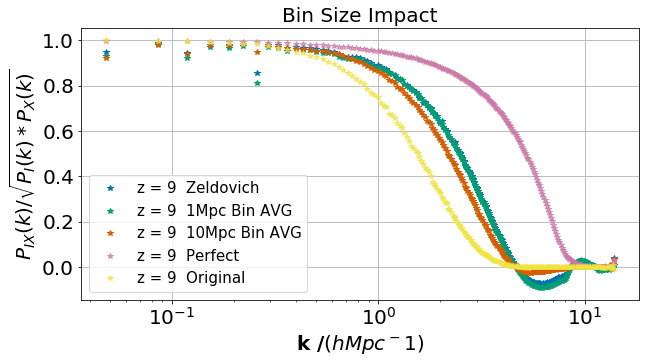
\includegraphics[width=1\columnwidth]{images/realRecon/binSize.png}%
    
    \caption{
    Normalized cross-spectra of realistic reconstructions with the initial field. This figure shows the impact of smoothing velocities over certain scales. Because we lose information by smoothing, the 10 Mpc reconstruction recovers less information compared to the 1 Mpc reconstruction. The Zel'dovich reconstruction is also present for comparison. As we are looking at reconstructions from $z=9$, they all work quite well because most particles are still in the quasi-linear regime.
    }
    
    \label{fig:4.2}
\end{figure}

Once we know the impact of the smoothing scale and that the reconstruction still performs very well when starting from $z=9$, we now want to compare their performance when starting from $z=0$. Figure~\ref{fig:4.3} shows the correlation between the $z=0$ field, reconstructed with the two methods, and the initial field. 

\begin{figure}
    \centering
    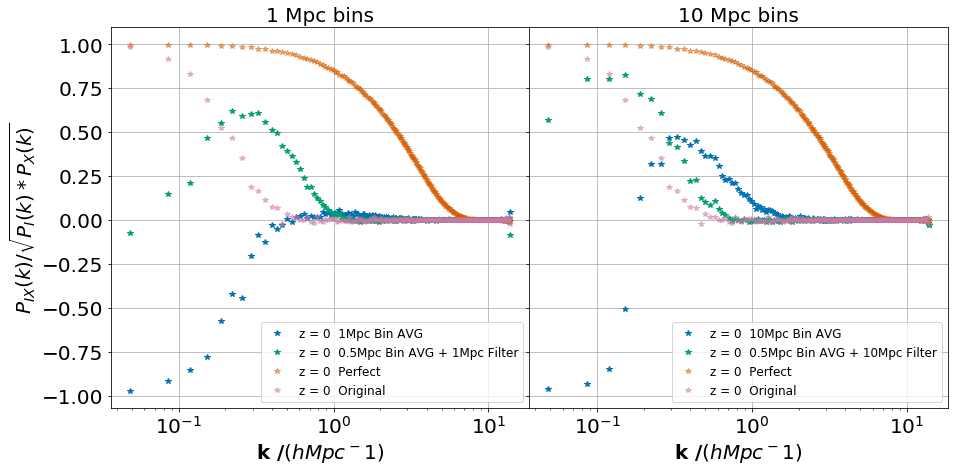
\includegraphics[width=1\columnwidth]{images/realRecon/filterComp.png}%
    
    \caption{
        Normalized cross-spectra of fields reconstructed from $z=0$ with the initial density field. We compare the two methods of smoothing velocities outlined in Section 3.2 for the two scales of interest. The left panel shows the comparison between the performance of the two methods when velocities are smoothed over 1 Mpc scales, while the right panel shows 10 Mpc scales. If we just average velocities over those scales, we still obtain an anti-correlation over the largest scales. However, when averaging over 0.5 Mpc scales and then applying a Gaussian Filter over the required scales, we see a large improvement in the reconstruction. An interesting effect is that for the 10 Mpc reconstructions, the first method slightly outperforms the second on intermediate scales. 
    }
    
    \label{fig:4.3}
\end{figure}

A normal velocity average over the interest scales produces results similar to what we found in Section 3.1 with the Zel'dovich reconstruction. We recover some information on intermediate scales, but the large scales become anti-correlated. Here, this seems to be taken to an extreme, in the sense that we have almost perfect anti-correlation on the largest scales. This result is very interesting and should be studied further in the future.

On the other hand, when we use smaller bins and a Gaussian filter, we get a much better correlation. We recover quite a bit of information over intermediate to large scales. However, the largest scales still seem to decorrelate. We will investigate this further in the next section where we compare results from different simulations. 

We found that using a Gaussian filter to smooth velocities works much better than normal averaging within the Zel'dovich reconstruction. This indicates that just averaging velocities in a 1 Mpc or even a 10 Mpc bin is not enough to bring us back into the quasi-linear regime. We do see an improvement in the reconstruction of intermediate scales when going from 1 Mpc to 10 Mpc averaging, but it still leads to an anti-correlation of the large scales.

An interesting outcome of these procedures is also the fact that for a small region, on intermediate scales (for 10 Mpc reconstructions), we do obtain a better correlation using normal averaging. This is probably an indication that we are losing more information when we smooth the field with a Gaussian filter. However, this method works up to much larger scales. By taking into account velocities of particles further away than the scale of interest (even though they have a small weight) we are getting closer to the quasi-linear regime. 

\subsection{Simulation comparison}

\begin{figure}
    \centering
    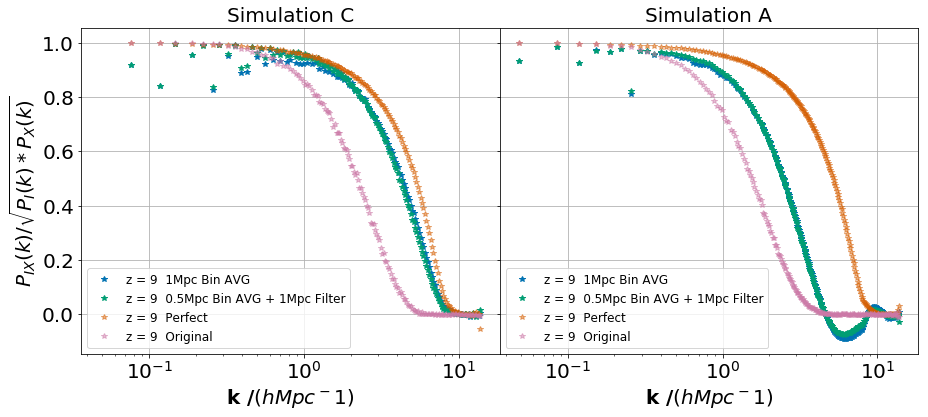
\includegraphics[width=1\columnwidth]{images/realRecon/z9SimComp.png}%
    
    \caption{
        Normalized cross-spectra of reconstructed $z=9$ fields with the initial field. We compare the same reconstruction methods (1 Mpc smoothing only) applied to two different simulations. On the left is Simulation C with a size of $(100$ Mpc$)^3$ and on the right is simulation A with a size of $(200$ Mpc$)^3$. The reconstruction in the smaller simulation recovers a lot more information, bringing the correlation very close to the perfect reconstruction.
        }
        
        \label{fig:4.4}
    \end{figure}
    
We now turn our attention to how these methods work when we apply them to different simulations. We have so far only looked at results from Simulation A, as it is the largest one and it has the best resolution. Figure~\ref{fig:4.4} presents the correlation of the $z=9$ reconstructed field with the initial density field in Simulation C and Simulation A. It shows that we are recovering information up to a smaller scale in the smaller simulation (C). This is not entirely surprising, as the smaller simulation is better correlated to begin with (as discussed in Chapter 2). What is surprising is how close to the perfect reconstruction the correlation gets.

The best overall correlation when reconstructing the $z=0$ density field was achieved in Simulation B. This result is shown in Figure~\ref{fig:4.5}. Both the 1 Mpc and the 10 Mpc reconstructions achieve a better correlation than the original on most scales. This simulation also gives us the best solution from a practical standpoint. When we calculate the average velocity field using $(0.5$ Mpc$)^3$ bins we have, on average, about 0.25 particles per bin. This means that most of our bins are actually empty, which for such small bins is exactly the case for observers as well. This is in contrast with simulation A, which has about 2 particles per bin.

\begin{figure}
    \centering
    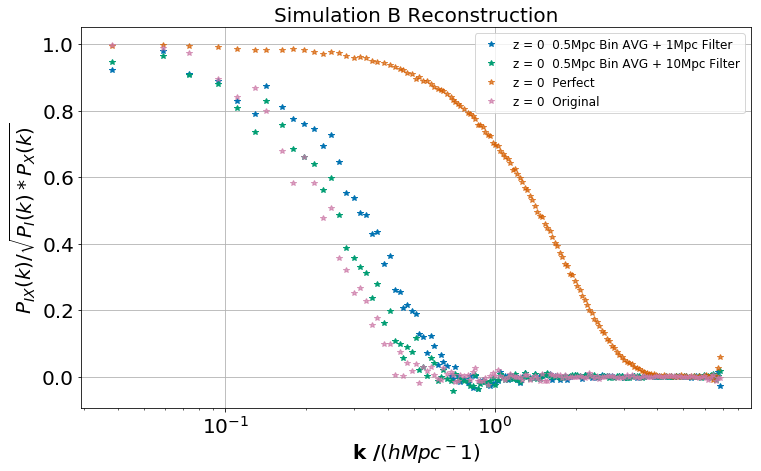
\includegraphics[width=1\columnwidth]{images/realRecon/simBRecon.png}%
    
    \caption{
        Normalized cross-spectra of the $z=0$ reconstructed fields with the initial density field within Simulation B. Our reconstruction methods work very well in this low resolution simulation in the sense that we don't destroy the correlation that was there to begin with (the largest scales). We also recover some information on intermediate scales, however, it is very far away from the perfect reconstruction. Also, we again encounter the effect found in Section 3.3.1: we recover less information when we smooth velocities over 10 Mpc compared to 1 Mpc. 
    }
    
    \label{fig:4.5}
\end{figure}

The best results for Simulation A are presented in Figure~\ref{fig:4.6}. Compared to Simulation B, we recover more information on intermediate scales. However, the largest scales decorrelate. There is also a larger difference between using a 1 Mpc and a 10 Mpc smoothing range. When using a 10 Mpc filter, we recover less intermediate scale information, but the large scales are much better correlated. This is a very good showcase for a trend we have been seeing in this chapter. When we choose to smooth the velocity field we are giving up some information in the hope of recovering the linear regime. The more velocity information we use, the more we destroy the large scale correlation by using the Zel'dovich approximation. However, using more velocity information generally leads to a better reconstruction on intermediate scales. This is an interesting information trade-off. The more intermediate scale information we recover, the more large-scale information we lose.


\begin{figure}
    \centering
    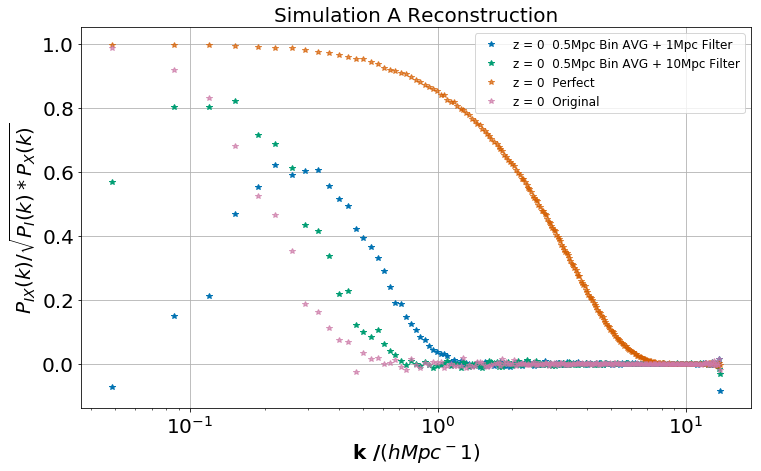
\includegraphics[width=1\columnwidth]{images/realRecon/simARecon.png}%
    
    \caption{
        Normalized cross-spectra of the $z=0$ reconstructed field with the initial density field within Simulation A. By smoothing velocities over 10 Mpc scales, we achieve a better correlation of the large scales, however we have a worse correlation over intermediate scales. The result for the intermediate scales was discussed in section 3.3.1. It is an outcome of the information lost when smoothing velocities. The interesting result is that within the Zel'dovich approximation, we manage to preserve the large scale correlation only by using less velocity information.
    }
    
    \label{fig:4.6}
\end{figure}

On the other hand, based on these results, a case could be made that by using less velocity information, we are just pushing the problem to larger scales. We still see the largest scales start to decorrelate even when using the Gaussian filter. If we had a much larger simulation with the same resolution we might still see the largest scales become anti-correlated. However, our initial goal was to study reconstruction on scales smaller than the BAO. In that respect, our methods do succeed, as we see an improvement in correlation on intermediate scales.

These results are still quite far away from the correlation we obtain with the perfect reconstruction. However, we only studied reconstructions within the Zel'dovich approximation. Higher orders of Lagrangian Perturbation Theory might be able to get us closer to the perfect reconstruction, and also solve the problem with the information trade-off. 

% \begin{figure}
%     \centering
%     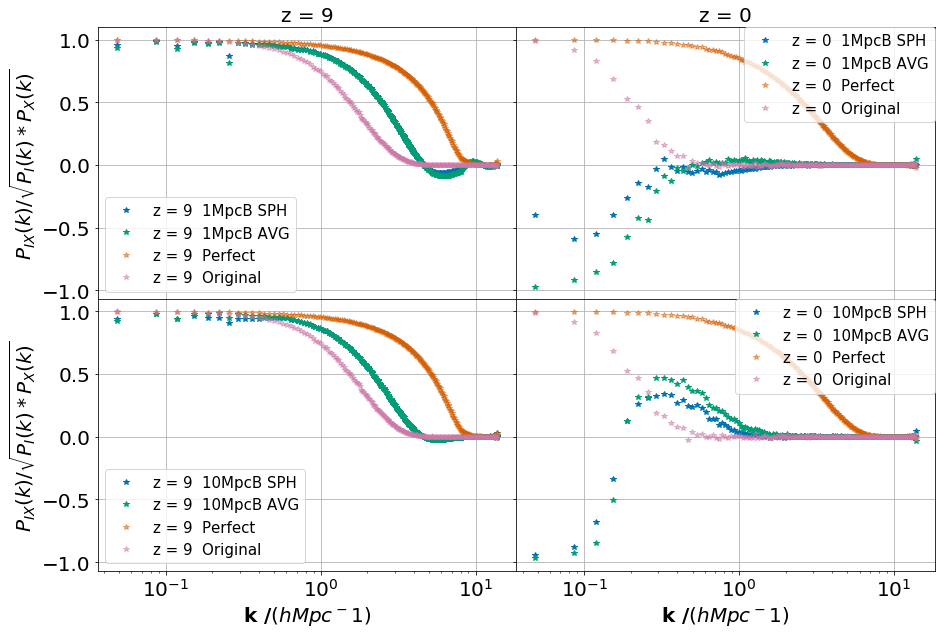
\includegraphics[width=1\columnwidth]{images/realRecon/sphVsAvg.png}%
    
%     \caption{
%     Cross spectra of realistic reconstructions from redshift 9 and 0, using 1 Mpc and 10 Mpc bins to average velocities. There are two averaging methods used: AVG - average of all particles in each bin, SPH - A point estimate of the velocity at the center of the bin.  
%     }
    
%     \label{fig:8}
% \end{figure}